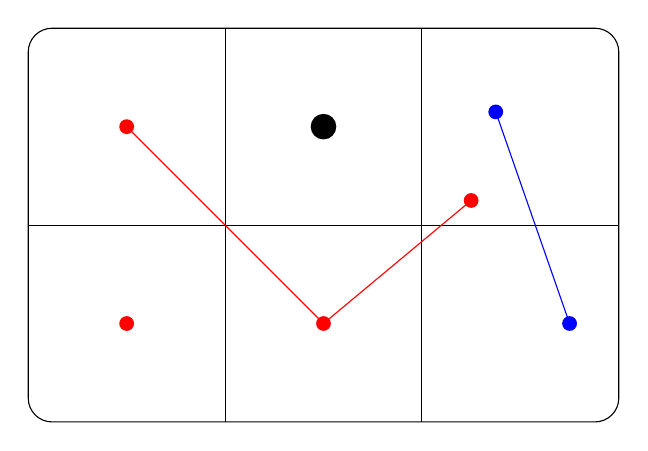
\begin{tikzpicture}[scale=1.25, every node/.style={scale=0.75}]
    \def\spnt{0.075} % Size of smaller points
    \def\lpnt{0.13} % Size of larger points
    \draw[rounded corners=2ex] (0,0) rectangle (6,4);
    \draw (2.0, 4) -- (2.0, 0);
    \draw (4.0, 4) -- (4.0, 0);
    \draw (0, 2) -- (6.0, 2);
    \fill[red] (1, 3) circle (\spnt);
    \fill[red] (1, 1) circle (\spnt);
    \fill[red] (3, 1) circle (\spnt);
    \fill[red] (4.5, 2.25) circle (\spnt);
    \draw[red] (1, 3) -- (3,1) -- (4.5,2.25);
    \fill (3,3) circle (\lpnt);
    \draw[blue] (4.75, 3.15) -- (5.5,1);
    \fill[blue] (4.75, 3.15) circle (\spnt);
    \fill[blue] (5.5, 1) circle (\spnt);
\end{tikzpicture}